%%% Esqueleto base de la presentacion
%%% No agregar las paginas con un include
%%% Lo que quieran aportar deben ser usuarios del TRAC

\documentclass{beamer}
\usepackage[spanish,activeacute]{babel}
\usepackage[utf8]{inputenc}
\usepackage{listings}
\usepackage{color}
\definecolor{gray2}{rgb}{100,100,100}
\definecolor{red}{rgb}{255,0,0}
\definecolor{green}{rgb}{0,1,0} 
\definecolor{blue}{rgb}{0,0,1} 
\newcommand{\blue}{\textcolor{blue}}
\newcommand{\red}{\textcolor{red}}
\newcommand{\green}{\textcolor{green}}



\usetheme[pageofpages=of,% String used between the current page and the
                         % total page count.
          alternativetitlepage=true,% Use the fancy title page.
          titlepagelogo=img/cti_hpc-500,% Logo for the first page.
          watermark=img/cti_hpc-500-off,% Watermark used in every page.
          watermarkheight=60px,% Height of the watermark.
          watermarkheightmult=2,% The watermark image is 4 times bigger
                                % than watermarkheight.
          ]{Torino}

\usecolortheme{nouvelle}
\vspace{-0.5cm}
\author{\large Cristián D. Maureira Fredes\\\normalsize \textcolor{gray}{cmaureir@csrg.inf.utfsm.cl}}
\title{\Huge Simulación de n-cuerpos}
\subtitle{\Large Un acercamiento utilizando paralelismo en CPU y GPU}
\institute{Universidad Técnica\\ Federico Santa María}

\begin{document}
\begin{frame}[t,plain]
\titlepage
\end{frame}

\section{Motivación}
\frame
{
\frametitle{Motivación}
\begin{columns}
  \begin{column}{0.5\textwidth}
	\begin{itemize}
		\item Astronomía.
		\begin{itemize}
			\item ALMA-UTFSM
		\end{itemize}
		\item GPU.
		\begin{itemize}
			\item Curso 2010-2
		\end{itemize}
		\item PASI.
		\begin{itemize}
			\item Presentaciones Hamada/Cruz.
			\item \textit{Nagasaki University}.
		\end{itemize}
	\end{itemize}
  \end{column}
  \begin{column}{0.5\textwidth}
	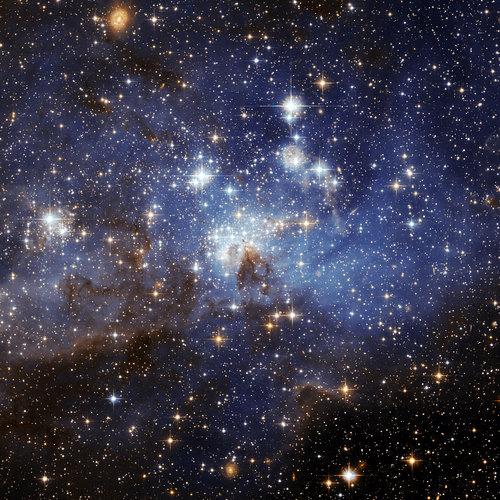
\includegraphics[width=0.8\textwidth]{img/stars}
  \end{column}
\end{columns}
}

\section{Trabajo}

\frame
{
\frametitle{Trabajo}
\framesubtitle{Problema de n-cuerpos}
\begin{block}{Definición}
	Predecir el \underline{movimiento} de un grupo de \underline{objetos celestes},
	que van \underline{interactuando} unos con otros gravitacionalmente.
\end{block}
}

\frame
{
\frametitle{Trabajo}
\framesubtitle{Simulación de n-cuerpos}
\begin{itemize}
	\item Simulación de un sistema dinámico de partículas.
	\item Aplicaciones
	\begin{itemize}
		\item Formación de estructuras no lineales.
		\begin{itemize}
			\item Filamentos de galaxias.
			\item Halos de galaxias.
		\end{itemize}
		\item Dinámica de ``Star clusters''.
		\item Movimiento de planetas.
		\item etc.
	\end{itemize}
\end{itemize}
}

\frame
{
\frametitle{Trabajo}
\framesubtitle{Algoritmo}
Secciones críticas:
\begin{columns}
	\begin{column}{0.5\textwidth}
		\begin{itemize}	
			\item Posiciones iniciales.
			\begin{itemize}
				\item \red{Random.}
				\item Plummer Model.
			\end{itemize}
			\item Método de integración.
			\begin{itemize}
				\item Euler.
				\item \red{Leapfrog.}
				\item Runge Kutta.
				\item Two step Adams-Bashworth.
				\item etc.
			\end{itemize}
		\end{itemize}
	\end{column}
	\begin{column}{0.5\textwidth}
		\begin{itemize}
			\item Cálculo de las fuerzas.
			\begin{itemize}
				\item \red{Particle-Particle.} \blue{$O(n^2)$}
				\item Particle-Mesh.  \blue{$O(n + ng\log ng)$}
				\item Treecode. \blue{$O(n\log n)$}
				\item Multipole. \blue{$O(n)$}
				\item etc.
			\end{itemize}
		\end{itemize}
	\end{column}
\end{columns}
}

\frame
{
\frametitle{Trabajo}
\framesubtitle{Algoritmo}

\begin{itemize}
	\item Cálculo de la fuerza.
	\begin{itemize}
		\item Posiciones iniciales $x_i$.
		\item Velocidades iniciales $v_i$.
		\item $1 \leq i \leq N$
	\end{itemize}
	$$f_{ij} =G \cdot \frac{m_i \cdot m_j}{||r_{ij}||^{2}} \cdot \frac{r_{ij}}{||r_ij||}$$
	\begin{itemize}
		\item $m_i$ y $m_j$ masas de los cuerpos $i$ y $j$.
		\item $r_{ij} = (x_j - x_i )$ vector de distancia entre los cuerpos $i$ y $j$.
		\item $G$, constante gravitacional. ($6,67428 \times 10^{-11} m^{3} kg^{-1} s^{-2}$)
	\end{itemize}
\end{itemize}
}

\frame
{
\frametitle{Trabajo}
\framesubtitle{Implementación}
\begin{columns}
	\begin{column}{0.5\textwidth}
		\begin{itemize}
			\item Serial.
			\item Paralela en CPU (OpenMP).
			\item Paralela en GPU (CUDA).
		\end{itemize}
	\end{column}
	\begin{column}{0.5\textwidth}
		
\includegraphics[width=0.5\textwidth]{img/openmp}
		
\includegraphics[width=0.5\textwidth]{img/nvidia}
	\end{column}
\end{columns}
}

\frame
{
\frametitle{Trabajo}
\framesubtitle{Resultados \blue{Serial}}
\begin{center}
	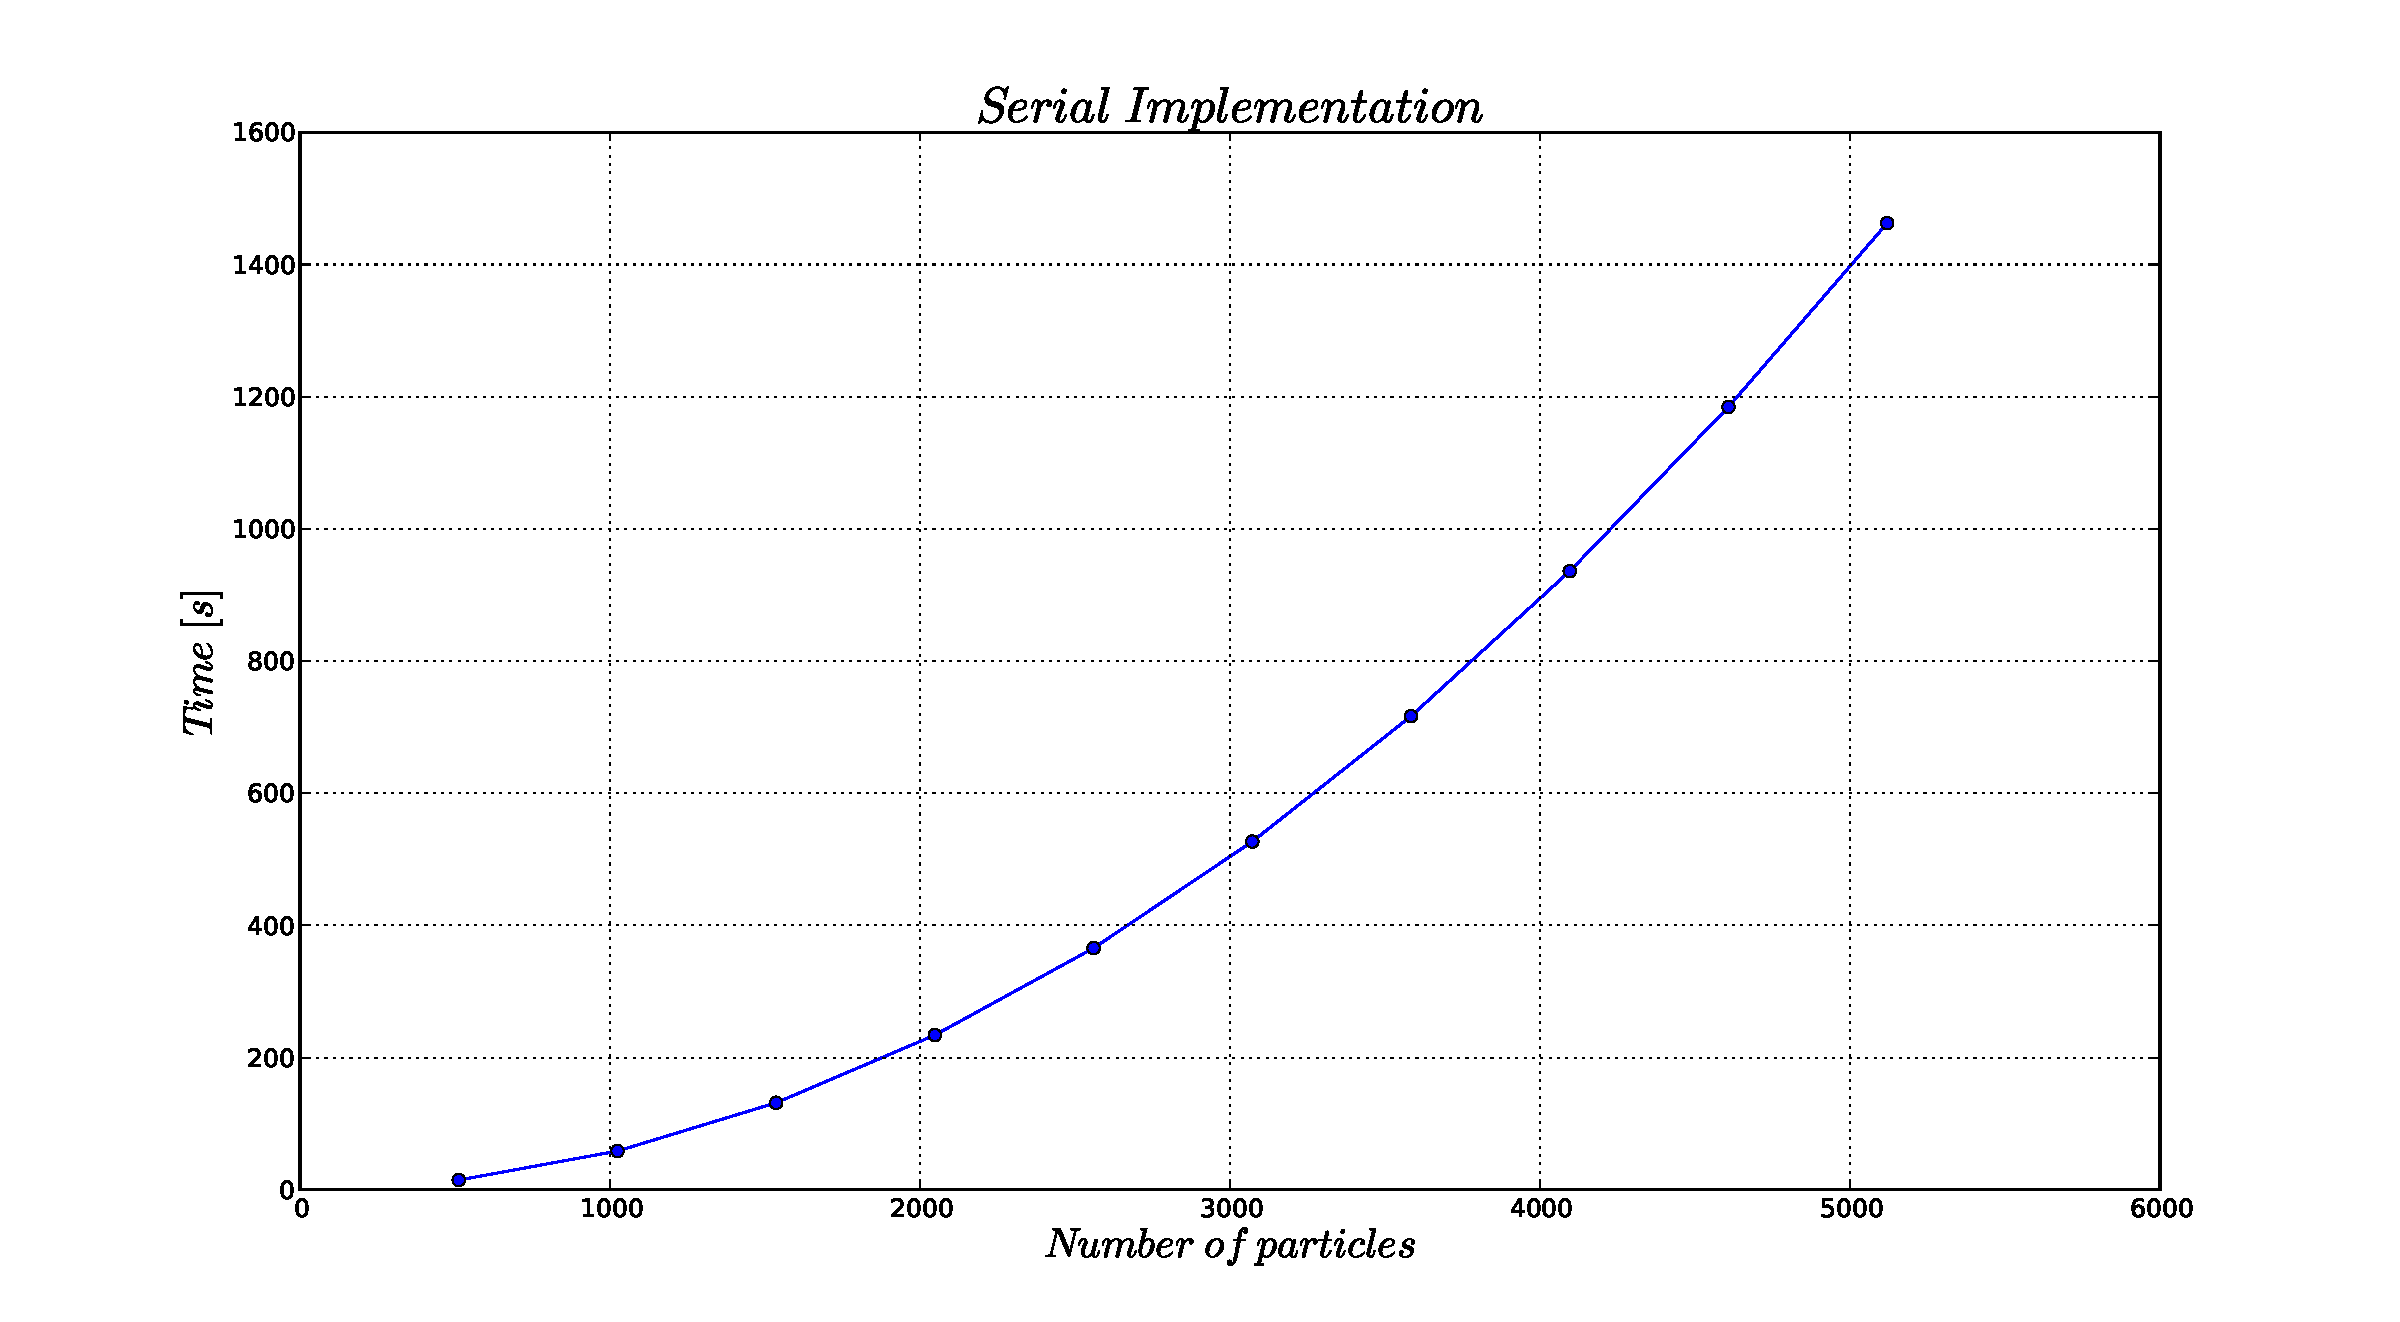
\includegraphics[width=0.95\textwidth]{img/serial.pdf}
\end{center}
}

\frame
{
\frametitle{Trabajo}
\framesubtitle{Resultados \blue{Serial}}
\begin{itemize}
	\item Tiempo cuadrático.
	\item Relación creciente.
\end{itemize}
}


\frame
{
\frametitle{Trabajo}
\framesubtitle{Resultados \blue{OpenMP}}
\begin{center}
	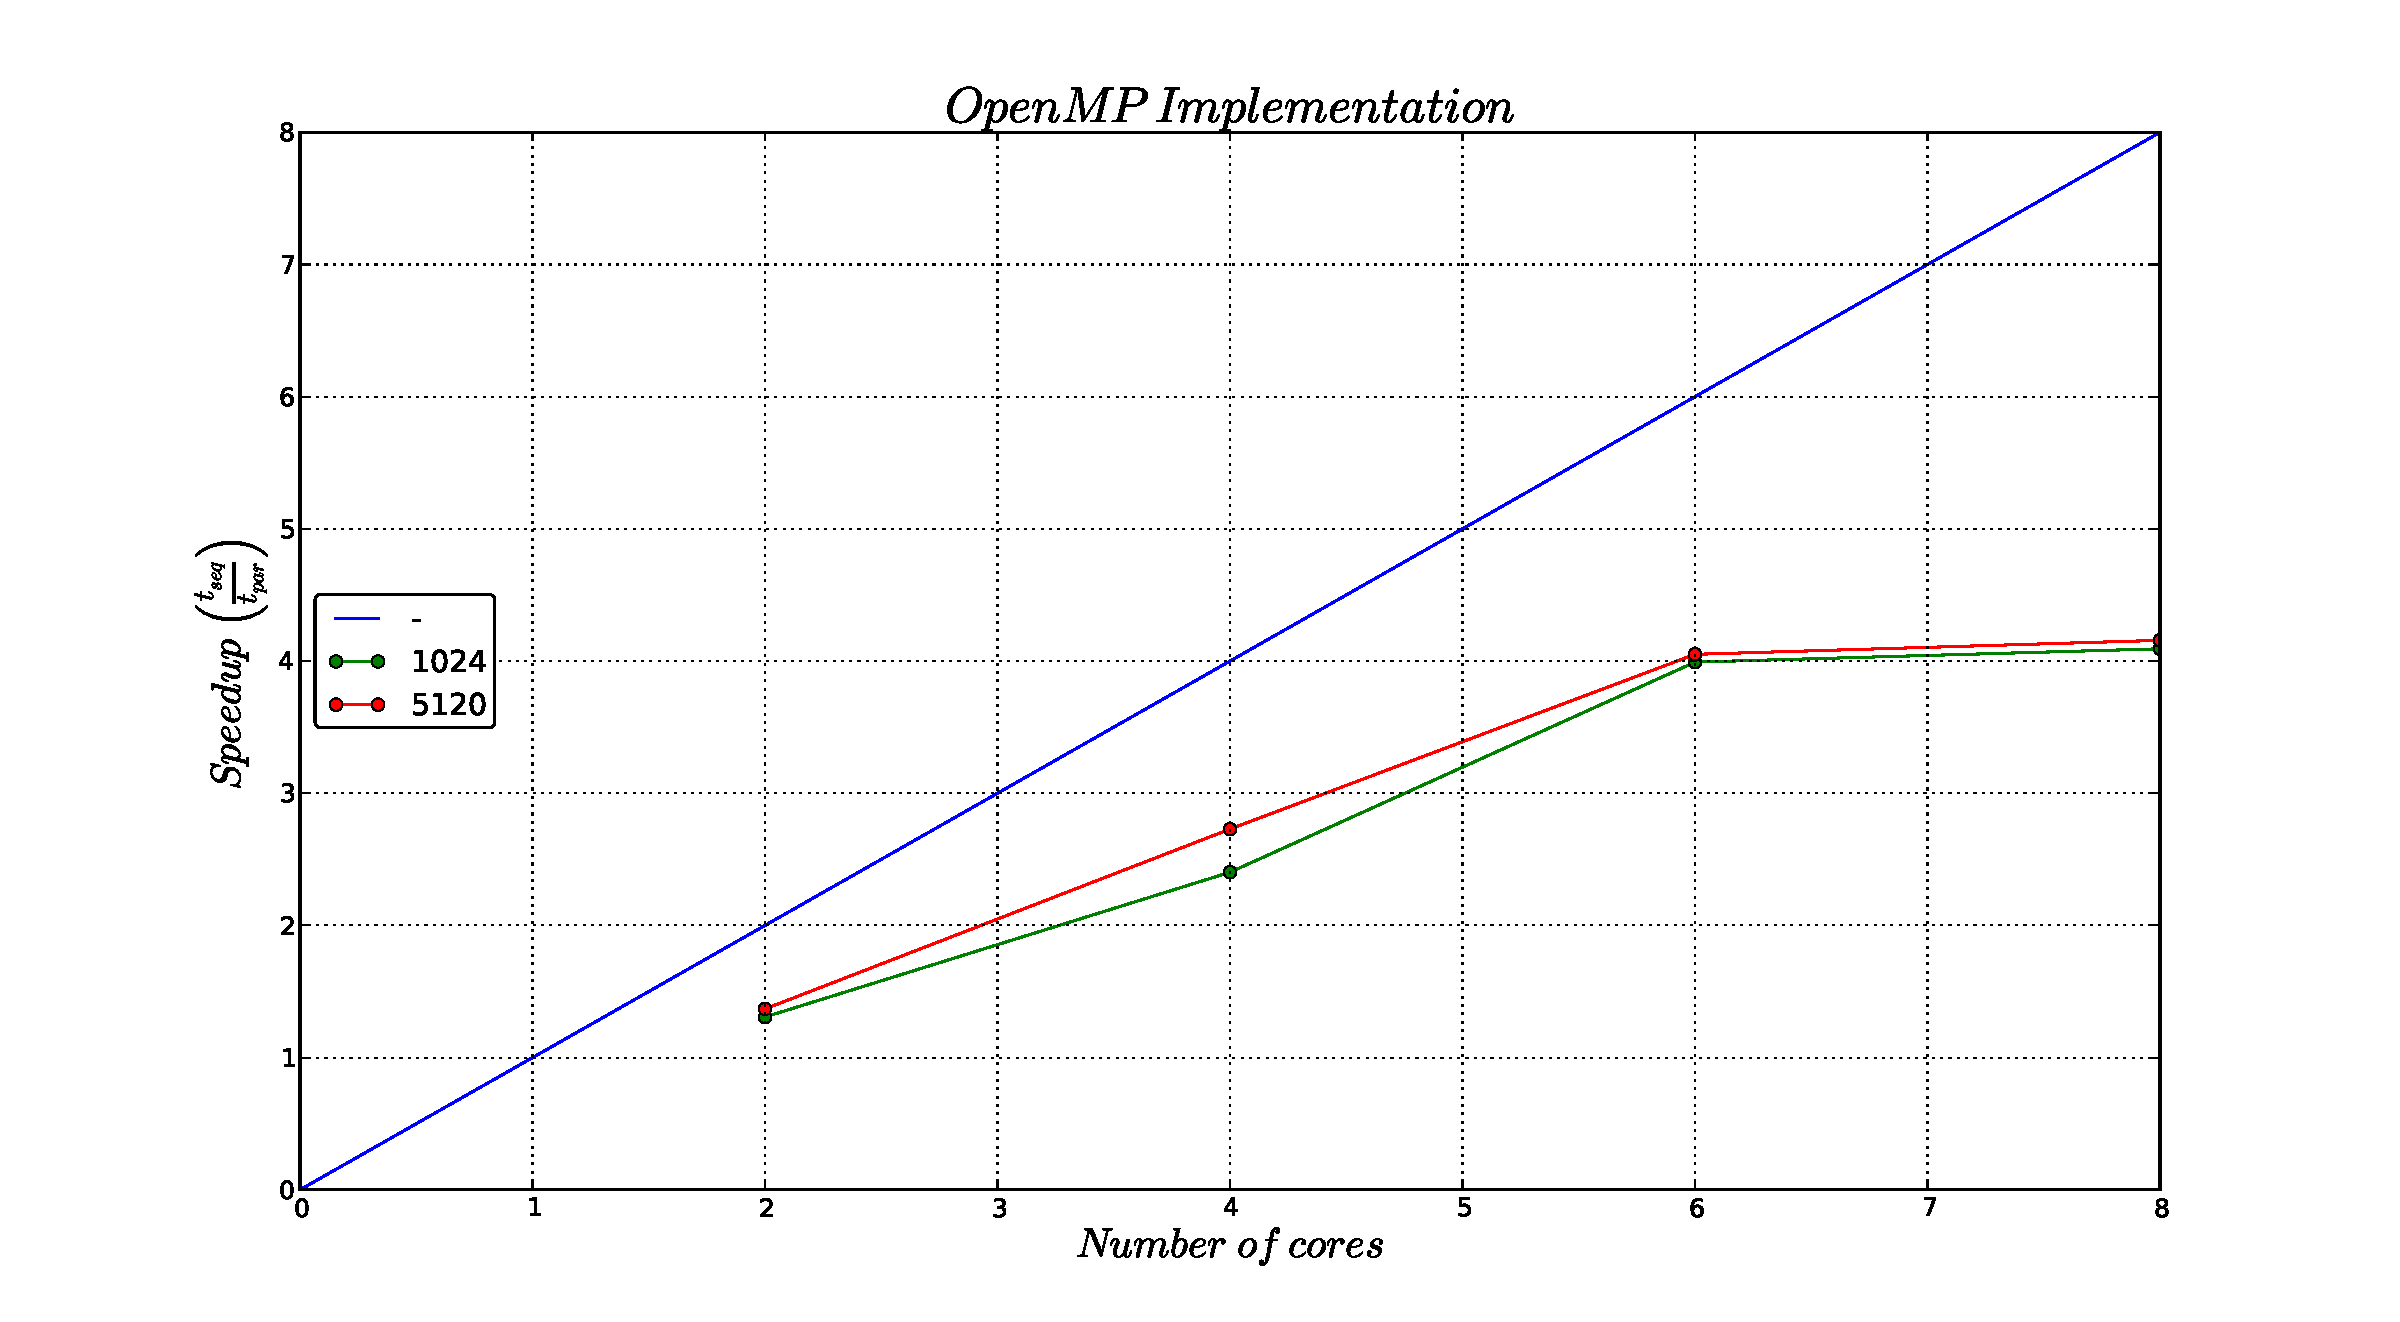
\includegraphics[width=0.95\textwidth]{img/openmp_speedup.pdf}
\end{center}
}

\frame
{
\frametitle{Trabajo}
\framesubtitle{Resultados \blue{OpenMP}}
\begin{itemize}
	\item Speedup $\approx$ 4x.
	\item Eficiencia $\approx$ 0.52\%.
	\item Escalabilidad aceptable hasta los 6 cores.
\end{itemize}
}

\frame
{
\frametitle{Trabajo}
\framesubtitle{Resultados \blue{CUDA}}
\begin{center}
	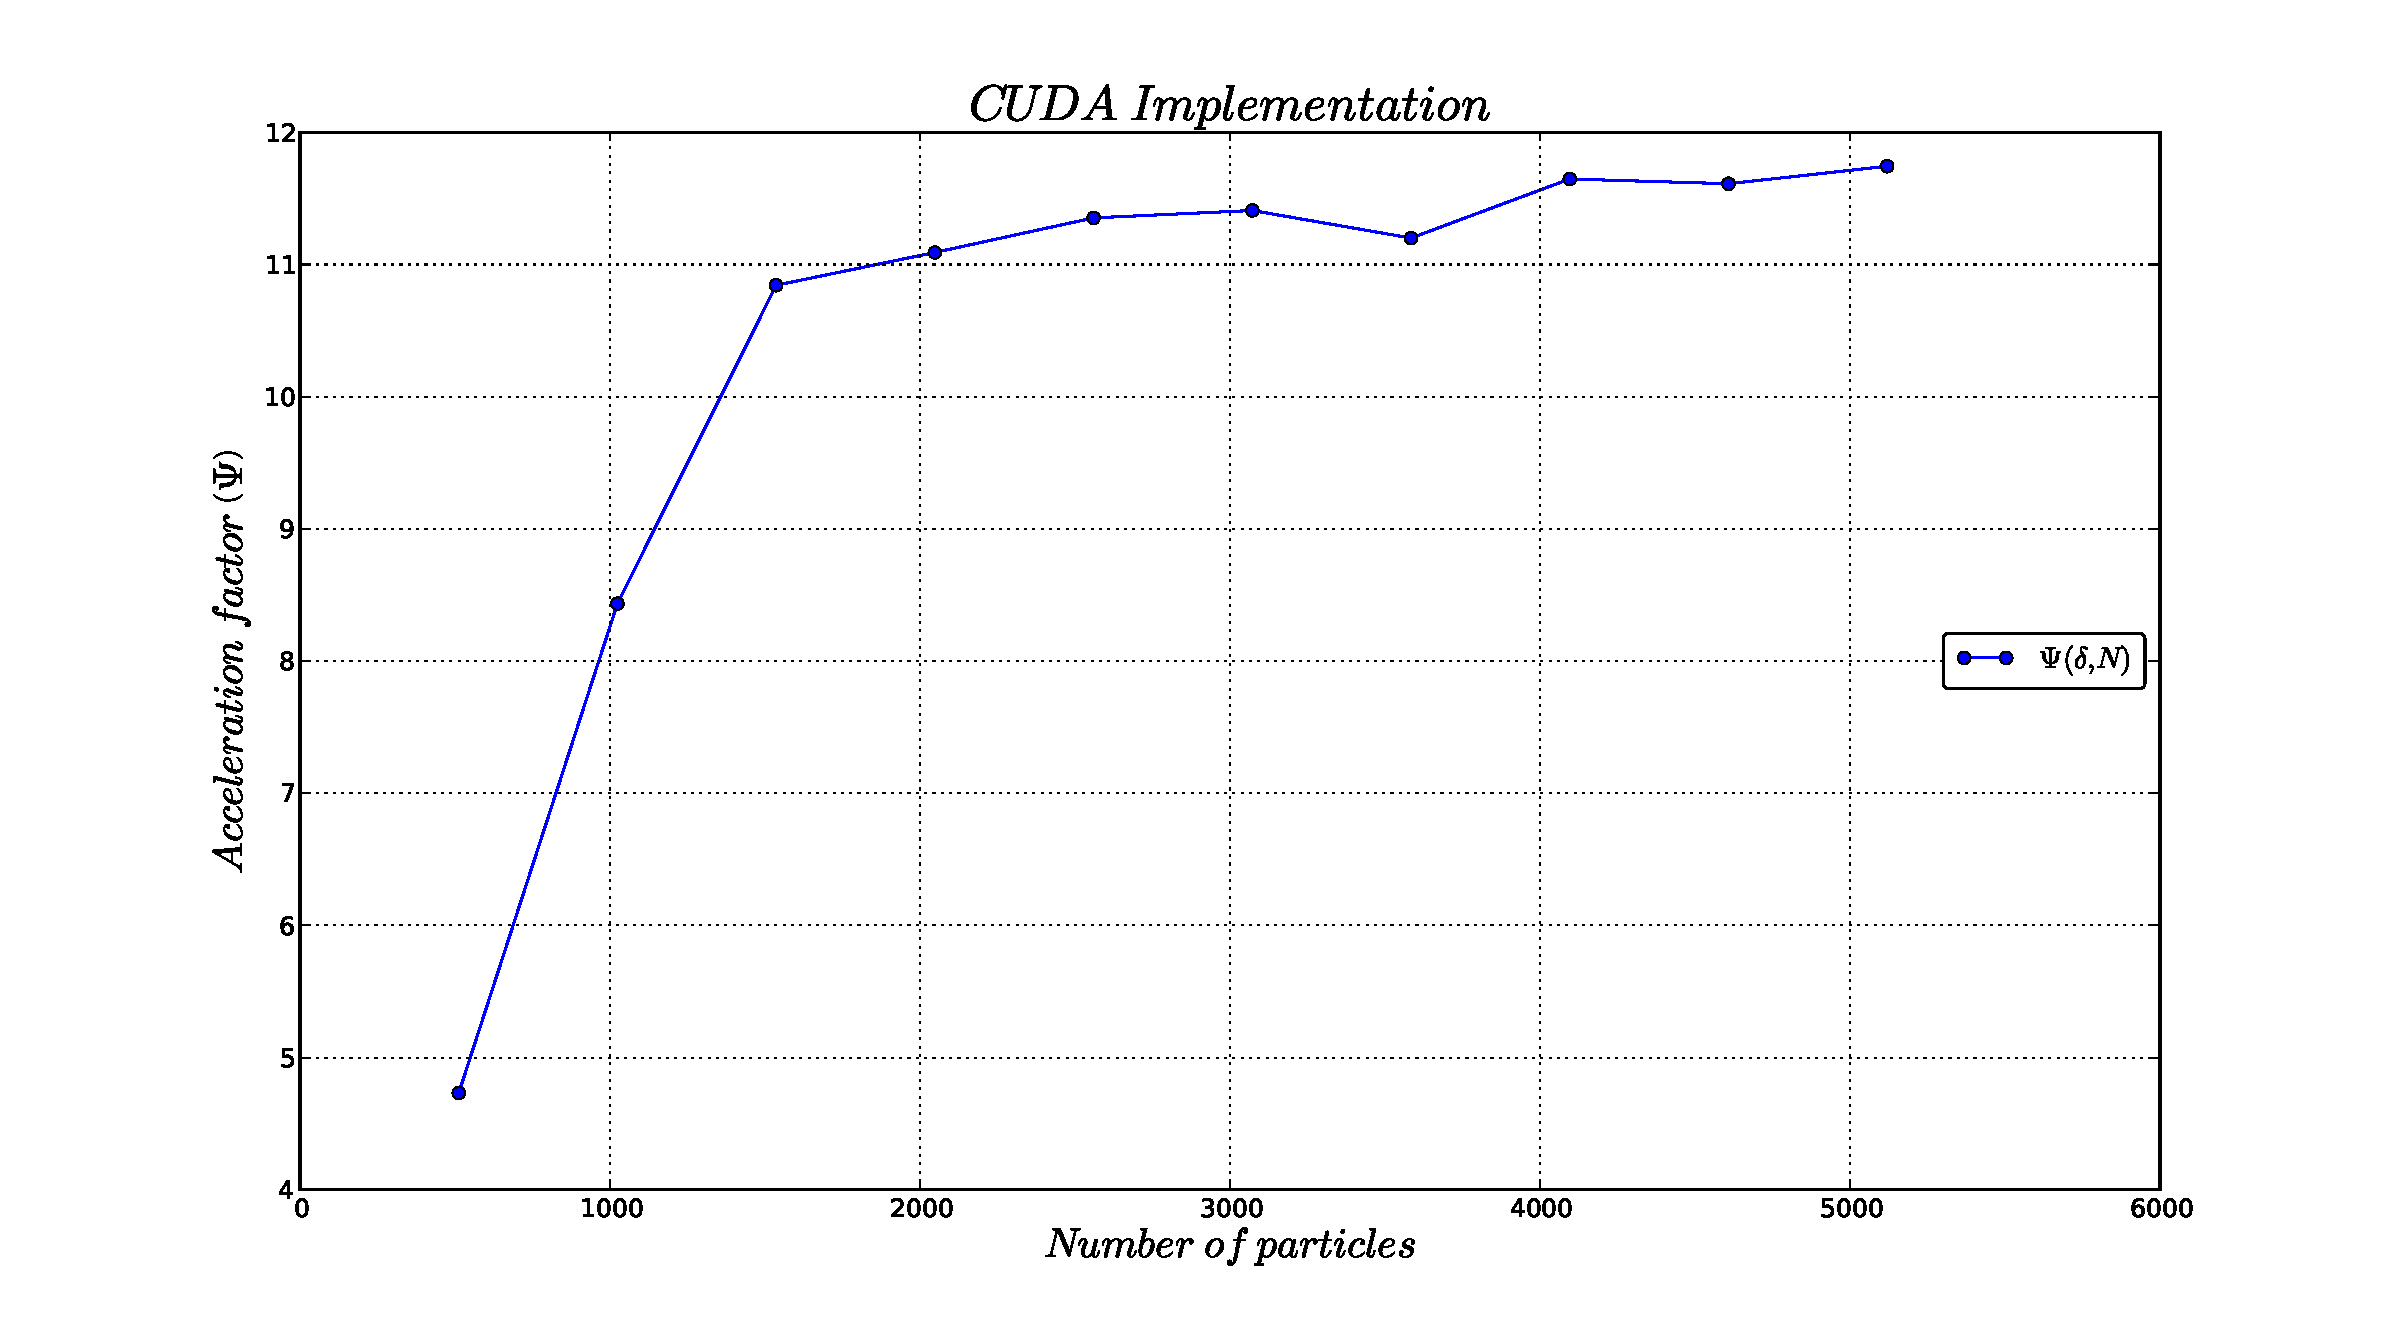
\includegraphics[width=0.95\textwidth]{img/cuda_speedup.pdf}
\end{center}
}

\frame
{
\frametitle{Trabajo}
\framesubtitle{Resultados \blue{CUDA}}
\begin{itemize}
	\item Speedup $\approx$ 11x.
%	\item Eficiencia $\approx$ ?
	\item Escalabilidad aceptable hasta 1536 particulas.
	\item Algoritmo favorece el utilizar más bloques y menos hebras.
\end{itemize}
}

\frame
{
\frametitle{Trabajo}
\framesubtitle{Resultados \blue{Tiempos}}
\begin{center}
	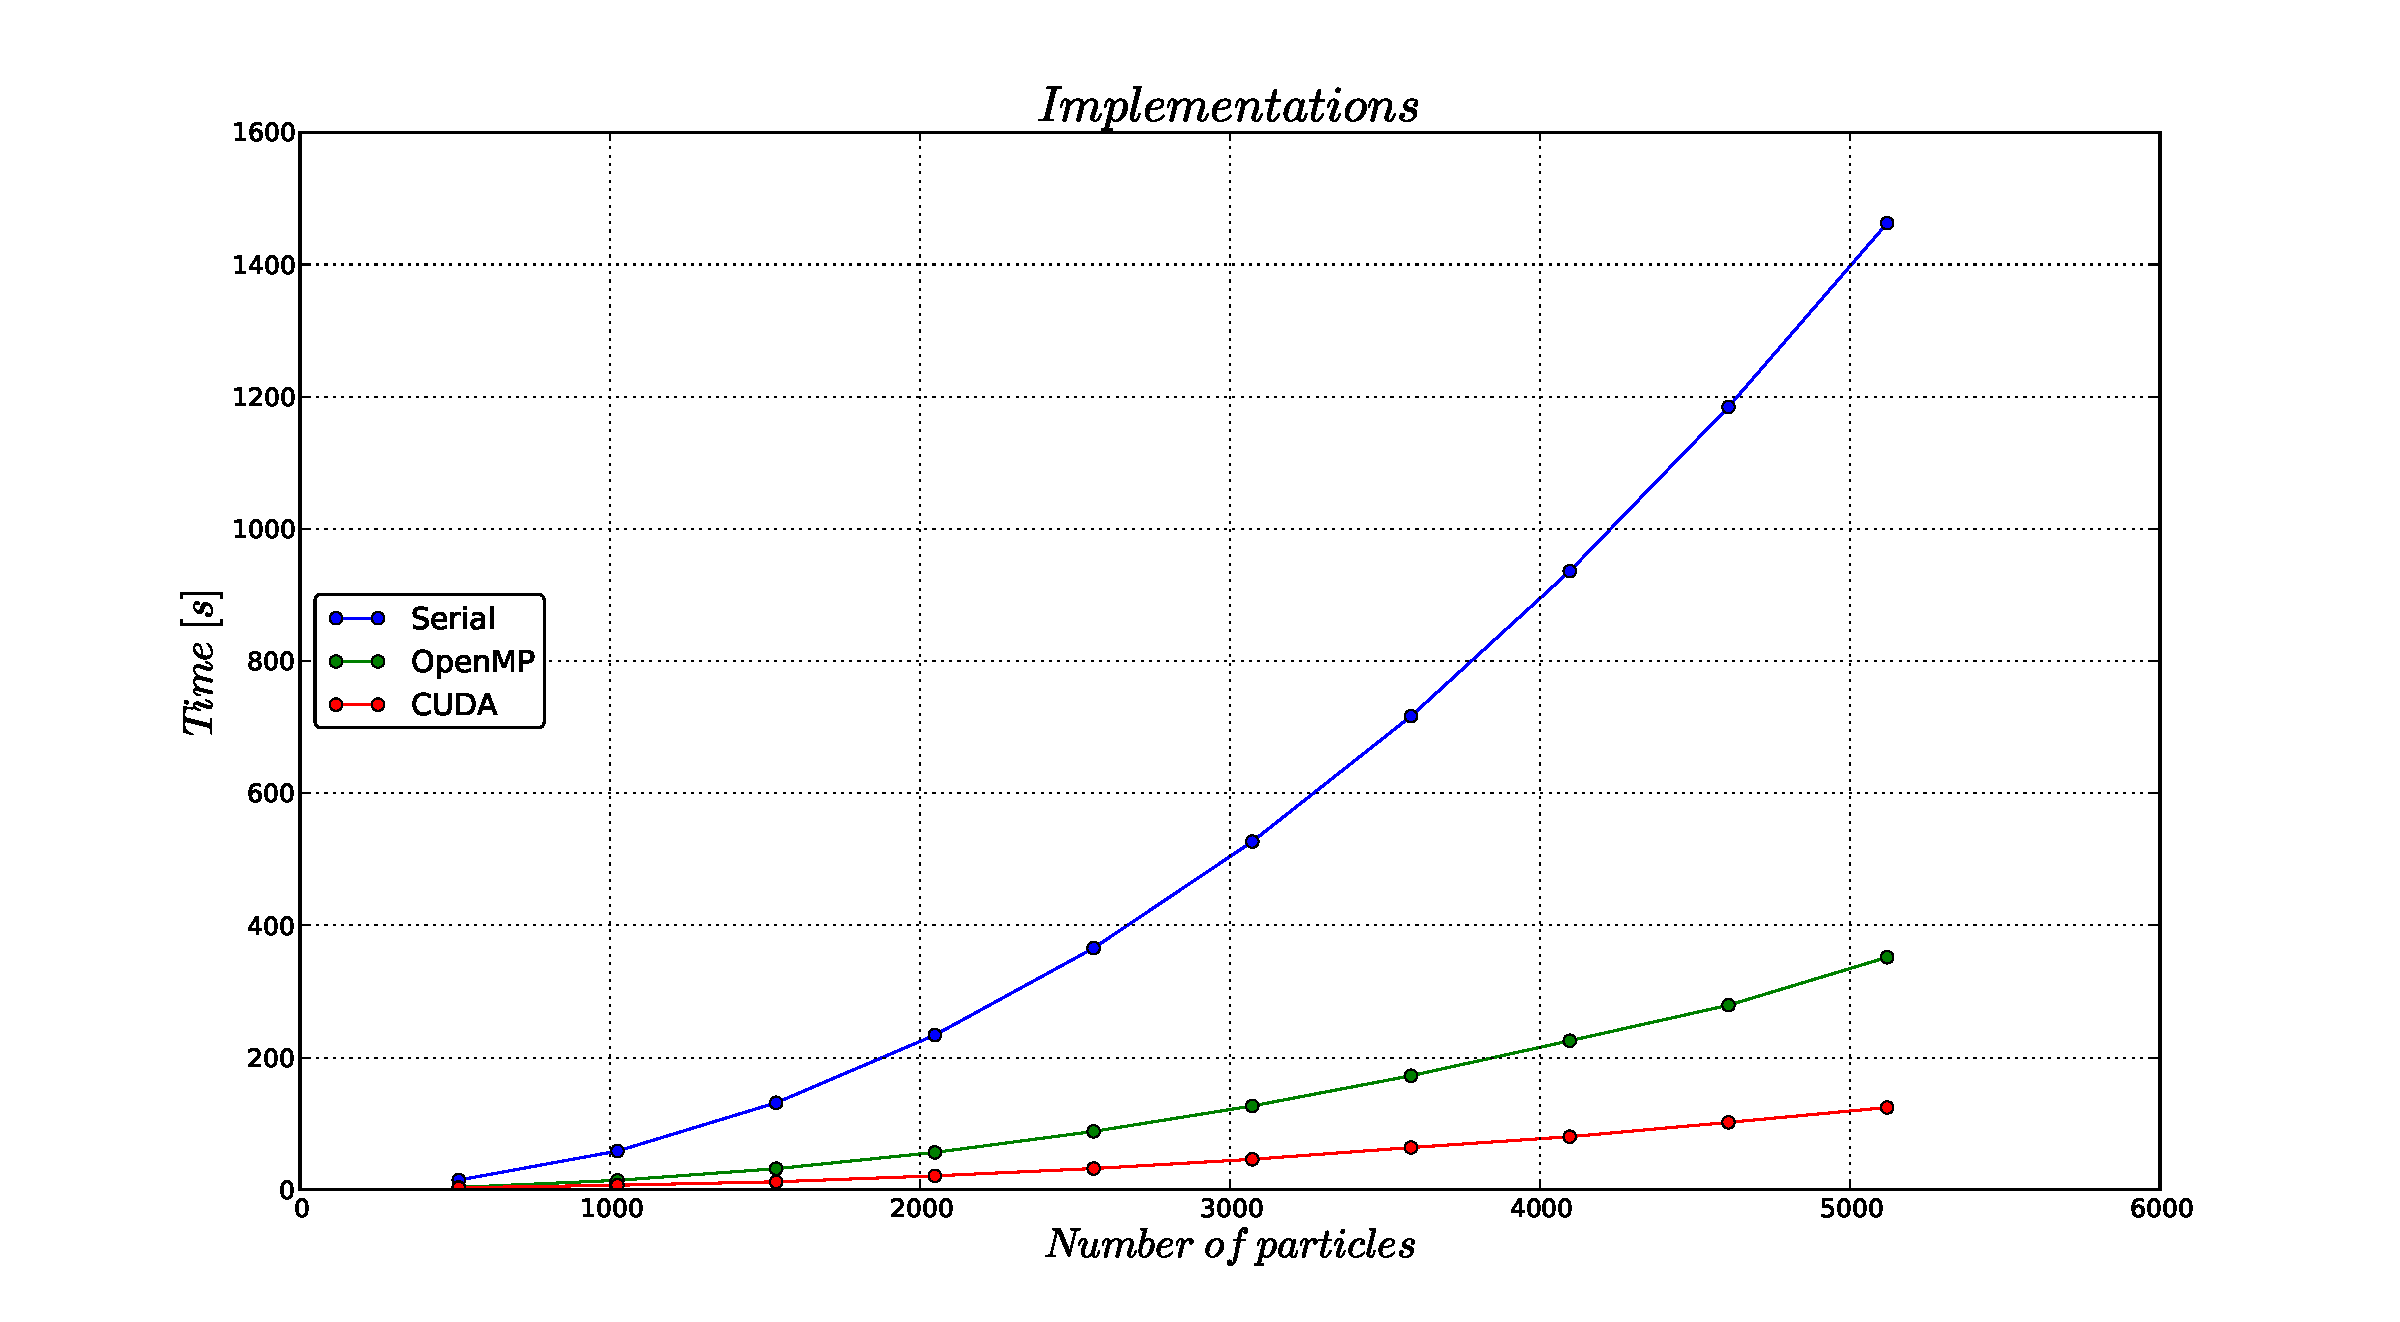
\includegraphics[width=0.95\textwidth]{img/all.pdf}
\end{center}
}

\frame
{
\frametitle{Trabajo}
\framesubtitle{Clases}

	\begin{columns}
	 	\begin{column}{0.5\textwidth}
			\begin{itemize}
				\item \textbf{Cesar Fernández}
				\item Computación paralela.
				\begin{itemize}
					\item Conceptos
					\item MPI
					\item OpenMP
				\end{itemize}
				\item Cluster
				\begin{itemize}
					\item Sistema PBS.
					\item Estructura cluster UTFSM.
					\item Scripts.
				\end{itemize}
				\end{itemize}
	 	\end{column}
	 	\begin{column}{0.5\textwidth}
			\begin{itemize}
				\item Evaluación paralelismo.
				\begin{itemize}
					\item Speedup y Eficiencia.
					\item Ley de Amdahl's.
					\item Ley de Gustafson-Barsis.
				\end{itemize}
			\end{itemize}
	 	\end{column}
	\end{columns}
}

\section{Conclusiones}
\frame
{
\frametitle{Conclusiones}
\framesubtitle{Literatura}
\begin{itemize}
	\item OpenMP
	\begin{itemize}
		\item ``The Art of concurrency: A Thread Monkey's Guide to Writing Parallel Applications'', (Clay Breshears).
		\item ``Using OpenMP: Portable Shared Memory Parallel Programming'', (Chapman et al.)
	\end{itemize}
	\item CUDA
	\begin{itemize}
		\item ``NVIDIA CUDA C Programming Guide''.
		\item ``NVIDIA CUDA C Best Practices Guide''.
	\end{itemize}
	\item Publicaciones.
\end{itemize}
}

\frame
{
\frametitle{Conclusiones}
\framesubtitle{Trabajo futuro}
\begin{itemize}
	\item Análisis de complejidad del algoritmo.
	\begin{itemize}
		\item Particle-Mesh
		\item Treecode.
	\end{itemize}
	\item Análisis de métodos de integración.
	\begin{itemize}
		\item Runge Kutta.
	\end{itemize}
	\item Análisis de posiciones iniciales.
	\begin{itemize}
		\item Plummer model.
	\end{itemize}
	\item Mejorar implementaciones.
\end{itemize}
}

\begin{frame}[t,plain]
\titlepage
\end{frame}

\end{document}
